\documentclass[tikz]{standalone}
\usepackage{tikz}
\usetikzlibrary{automata, positioning}

\begin{document}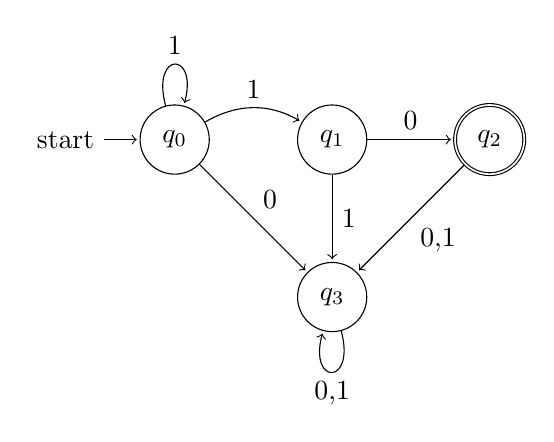
\begin{tikzpicture}[shorten >=1pt, node distance=2cm, on grid, auto]

\node[state, initial] (q0) {$q_0$};
\node[state] (q1) [right=of q0] {$q_1$};
\node[state, accepting] (q2) [right=of q1] {$q_2$};
\node[state] (q3) [below=of q1] {$q_3$};

\path[->]
  (q0) edge[loop above] node {1} ()
       edge[bend left] node {1} (q1)
       edge node {0} (q3)
  (q1) edge node {0} (q2)
  (q1) edge node {1} (q3)
  (q2) edge node {0,1} (q3)
  (q3) edge[loop below] node {0,1} ();

\end{tikzpicture}
\end{document}
